
\subsection{Overview}

This section outlines our approach. The overall methodology is illustrated in Figure \ref{fi:test}.

%Both static information and motion information, are correlated with the actions occurring in a video. For example, diving action
%is highly associated with swimming pools, and javelin throw is highly likely to happen in a scenario, where a sports field, a javelin and an athlete is
%present. Therefore, it is important to extract both static and motion information, in order to accurately predict and classify actions. In other words,
%individual objects, scene information, and actions and movements of actors and objects are extracted, in the process of prediction. 


%Also, a complex action may consist of smaller sub actions. For example, javelin throw action consists of sub events like getting ready,
%running, and throwing the javelin. Also, a specific order of sub events are associated with the complex action. 
%Therefore, it is important to investigate the evolution of sub activities with respect to time, in order to predict
%complex actions. We investigate this using following method. A video is segmented in to smaller segments, and features are engineered for each of these sub segments. A video can be then represented as a vector time series $C = [c_{t_0}, c_{t_1}, ...c_{t_{n-1}}]$.
%, where $n$ is the number of segments. Then, a recurrent neural net is applied on these features, to extract temporal dynamics.
\begin{figure*}
  \centering
  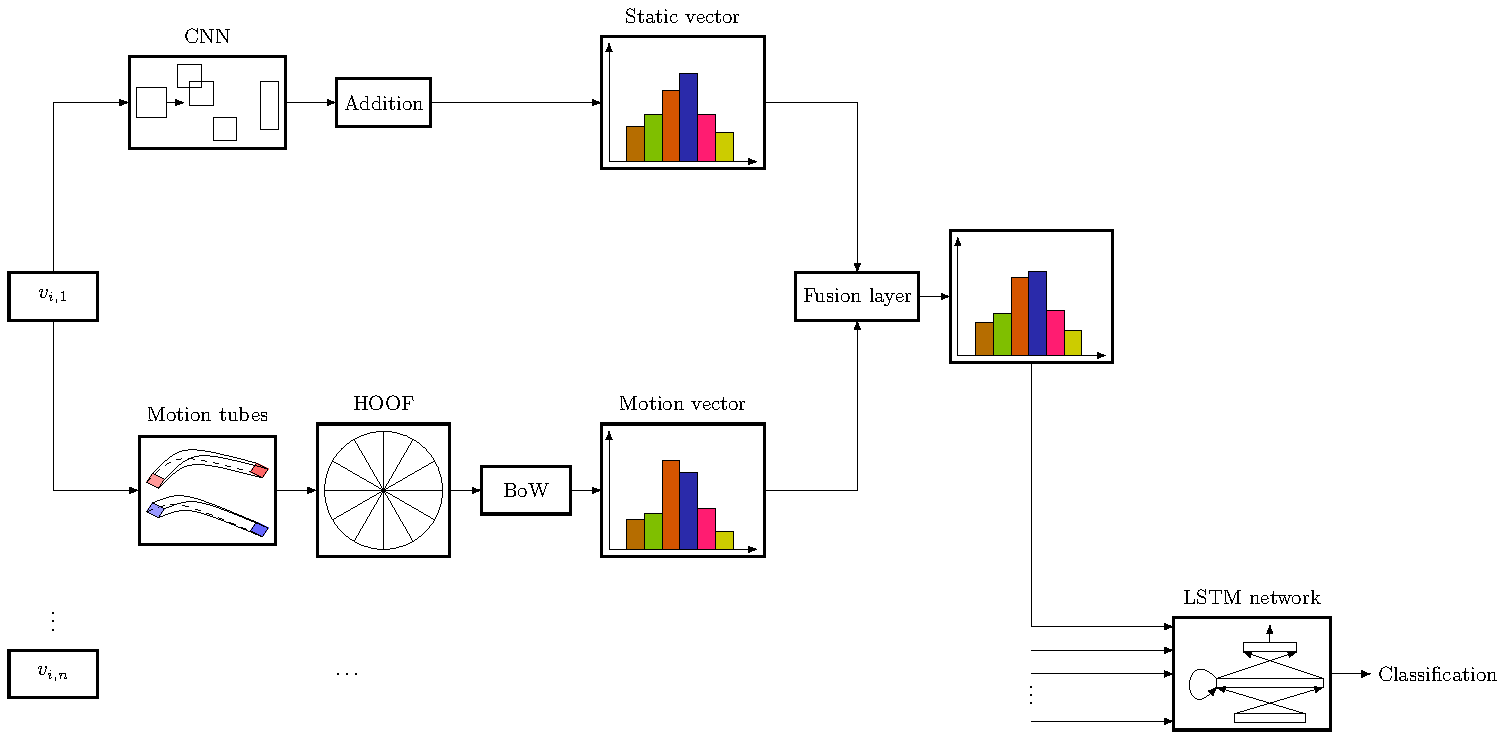
\includegraphics[width=18cm, height=6cm]{overall.pdf} 
  \caption{\textbf{Overall methodology}. The whole process consists of five major steps: (i) segmenting a video (ii) crafting static features, (iii) crafting motion features,
  (iv) fusing static and motion features, and (v) capturing temporal evolution of sub events. Static and motion features are independant 
  and complementery. We generate static and motion features based on a pre-trained CNN and
  motion tubes respectively, and capture the emporal evolution of sub events using a LSTM network.}
  
 \label{fi:test}
\end{figure*}


First, we segment a video in to smaller segments of 15 frames with a constant frame overlap
and carry out feature construction pipeline for each of these sub segments, as shown in Figure \ref{fi:test}. 
We create features for describing both motion and static domains.

For extracting motion features we create \textit{motion tubes} across frames, where we track each moving area along the frames using ``action boxes''.
Action boxes are square regions, which contain significant motion in each frame. We choose candidate areas by first creating dense trajectories for each frame,
and then clustering trajectory points proceeded by a significant amount of pre processing. This process is explained in sub section $B$.
These action boxes create motion tubes by linking across the frames. Then, we calculate (HOOF)\cite{chaudhry2009histograms} features within these motion tubes and apply a  
bag of features
method on these features to create a descriptor for each video segment. 

For extracting static features, we train a deep CNN, on Imagenet, and then apply this CNN,
on the frames of a video segment to retrieve deep features--output vector from the final softmax layer of the CNN---from it. Then, we use these features
to create a static descriptor for the video segment.

Afterwards, we combine these features, using one of the fusion models described in sub section $D$.

The system can then represent a video as a vector time series $C = [c_{t_0}, c_{t_1}, ...c_{t_{n-1}}]$,
where $n$ is the number of segments. Then, we apply a LSTM network on these features, and exploit the dynamics of time evolution of the combined vector.
Then, we classify the dynamics of this time series and predict actions.



